\documentclass[class=report, crop=false, 12pt,a4paper]{standalone}
\usepackage{float}
\usepackage{graphicx}
\usepackage{siunitx}
\usepackage{mathtools}
\usepackage{amsmath}
\usepackage{amssymb}
\usepackage{commath}
\usepackage[a4paper,width=150mm,top=25mm,bottom=25mm]{geometry}
\begin{document}
\section{The s-Plane - Poles and Zeroes}
\subsection{Example: Servo as a second order system}
\begin{figure}[H]
  \centering
  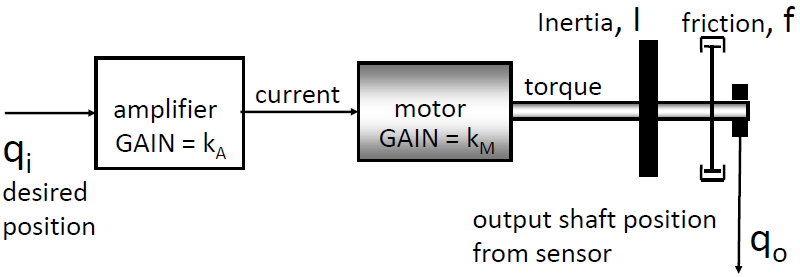
\includegraphics[width = 0.6\textwidth]{../img/diagram87.png}
\end{figure}
We saw last week that a DC motor servo with position control has a transfer function of a second order system.
\begin{figure}[H]
  \centering
  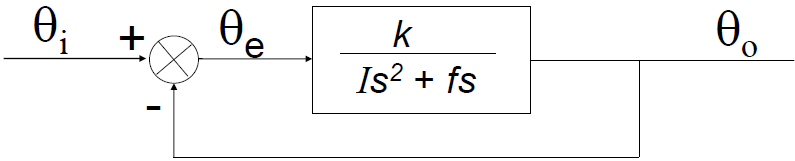
\includegraphics[width = 0.6\textwidth]{../img/diagram88.png}
\end{figure}
\begin{align}
  F(s) = \frac{G(s)}{1+G(s)} = \frac{\frac{K}{I}}{s^2 + \frac{f}{I}s + \frac{K}{I}}
\end{align}
Where, $\omega_n = \sqrt{\frac{k}{I}}$ (with increasing $k$, $\omega_n$ increases) and $\zeta = \frac{f}{2\sqrt{kI}}$ (with increasing $k$, $\zeta$ decreases).
\begin{figure}[H]
  \centering
  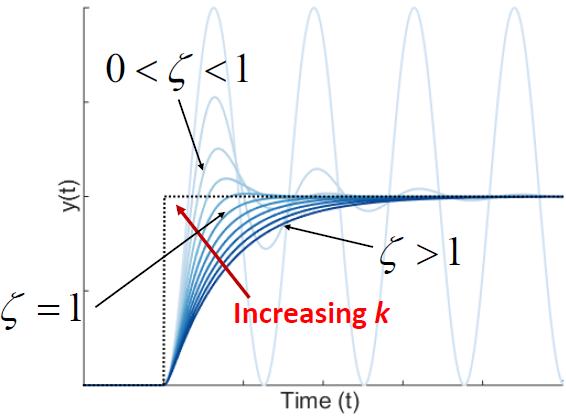
\includegraphics[width = 0.6\textwidth]{../img/diagram89.png}
\end{figure}
The overdamped ($\zeta > 1$) and critically damped ($\zeta = 1$) responses are seldom desirable for control systems due to their long settling time. $\zeta = 0.7$ gives a fast response without excessive overshoot or oscillations.
\subsection{Transfer functions}
As we have seen, transfer functions allow for important characteristics of the system response to be determined, without having to solve complete differential equations. Generally, transfer functions can be derived from the differential equations thusly: 
\begin{multline}
  a_n \frac{\dif^n y}{\dif t^n} + a_{n-1}\frac{\dif^{n-1} y}{\dif t^{n-1}} + ... + a_2 \frac{\dif^2 y}{\dif t^2} + a_1 \frac{\dif y}{\dif t} + a_0 y =\\ b_0 x + b_1 \frac{\dif x}{\dif t} + b_2 \frac{\dif^2 x}{\dif t^2} + ... + b_{m-1}\frac{\dif^{m-1} x}{\dif t^{m-1}} + b_m \frac{\dif^{m} x}{\dif t^m} \label{TFEq1}
\end{multline}
(Solving equation (\ref{TFEq1}) is hard!). Where $a$ are the output coefficients and $b$ are the input coefficients, combined these \textbf{entirely} characterise the system. The Laplace domain transfer function is then given by:
\begin{align}
  G(s) = \frac{b_m s^m + b_{m-1} s^{m-1} + ... + b_1 s + b_0}{a_n s^n + a_{n-1} s^{n-1} + ... + a_1 s + a_0}
\end{align}
\subsection{System poles and zeroes}
As defined, the transfer function is a rational function in the complex variable $s=\sigma + j\omega$, that is:
\begin{equation}
  G(s) = \frac{b_m s^m + b_{m-1} s^{m-1} + ... + b_1 s + b_0}{a_n s^n + a_{n-1} s^{n-1} + ... + a_1 s + a_0}
\end{equation}
It is often convenient to factor the polynomials in the numerator and denominator; and to write the transfer function in terms of those factors:
\begin{equation}
  G(s) = \frac{N(s)}{D(s)} = K\frac{(s-z_1)(s-z_2)...(s-z_{m-1})(s-z_m)}{(s-p_1)(s-p_2)...(s-p_{n-1})(s-p_n)}
\end{equation}
where the numerator and denominator polynomials, $N(s)$ and $D(s)$, have real coefficients defined by the system's differential equation. Poles and zeroes are found by:
\begin{equation}
  N(s) = 0 \textrm{ and } D(s) = 0
\end{equation}
All of the coefficients of polynomials $N(s)$ and $D(s)$ are real, therefore the poles and zeroes must be either purely real, or appear in complex conjugate pairs.
\begin{quotation}
  The poles and zeros are properties of the transfer function, and therefore of the differential equation describing the input-output system dynamics. Together with the gain constant, they completely characterise the differential equation and provide a complete description of the system.
\end{quotation}
\subsection{Transfer functions in the s-plane}
A system is characterised by its poles and zeroes as they allow the reconstruction of the input/output differential equation. It is possible to get a sense of the system dynamics from plotting the poles and zeroes graphically on the s-plane. A pole is commonly represented by a cross ($\times$) and a zero by a circle ($\circ$). Recall that, as $s$ is a complex number, we can plot the value on a plane, with a real and imaginary axis. 
\begin{equation}
  s = \sigma + j\omega
\end{equation}
By plotting the locations of the poles and zeroes on this plane, we can obtain a considerable amount of information about the response of the system without having to take the inverse Laplace transform. Each pole corresponds to a component of the time domain response, so from the plot it is possible to determine:
\begin{itemize}
  \item What components exist
  \item Their relative important (and possible simplifications)
  \item How they change with gain
\end{itemize}
\subsubsection{Real poles - exponentials}
First lets look at the real component only:
\begin{gather}
  s = \sigma\\
  e^s \rightarrow e^{-\sigma}
\end{gather}
Corresponding to $Ce^{-\sigma t}$
\begin{figure}[H]
  \centering
  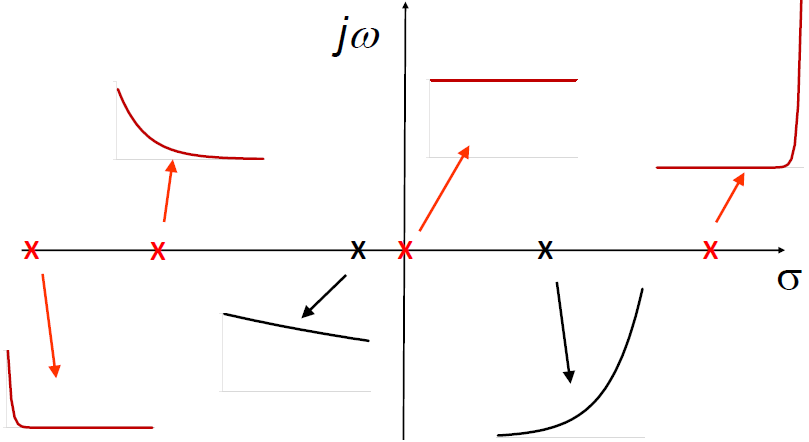
\includegraphics[width = 0.6\textwidth]{../img/diagram90.png}
\end{figure}
Poles located on the real axis have an exponential component only, with the pole location determining the rate of decay. Poles close to origin decay slowly, where poles far away decay rapidly. Poles located in the right hand side exponentially \textbf{increase}, whereas poles on the left hand side \textbf{decrease}. A pole on the origin is a flat 'DC' response.
\subsubsection{Imaginary poles - sinusoids}
First lets looks at the imaginary component only:
\begin{gather}
  s = \pm j\omega\\
  e^s \rightarrow e^{\pm j\omega}
\end{gather}
Which, from Euler's formula gives a sinusoidal response:
\begin{equation}
  e^{jx} = \cos{x} + j\sin{x}
\end{equation}
Poles located on the imaginary axis are in conjugate pairs.
\begin{figure}[H]
  \centering
  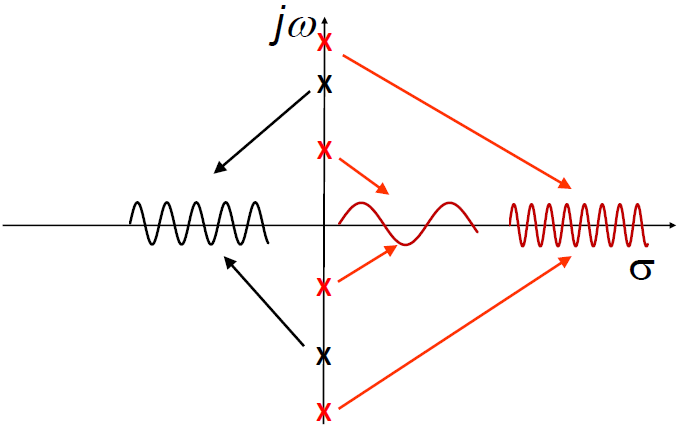
\includegraphics[width = 0.6\textwidth]{../img/diagram91.png}
\end{figure}
The imaginary poles generate an oscillatory component with a constant amplitude. Poles closer to the origin have a low frequency, which increases the further poles are from the origin.
\subsubsection{Complex poles}
Commonly, the poles are a combination of the two components.
\begin{figure}[H]
  \centering
  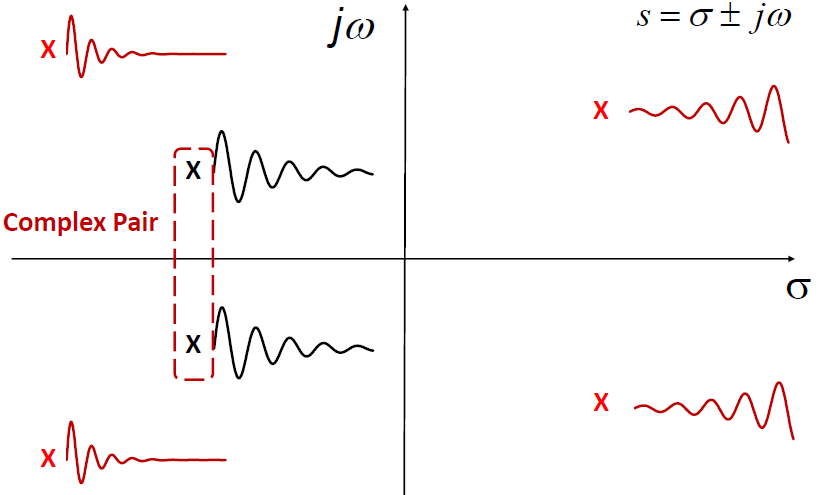
\includegraphics[width = 0.6\textwidth]{../img/diagram92.png}
\end{figure}
A complex conjugate pair of complex poles generates an exponentially decaying sinusoid in the form: 
\begin{equation}
  Ae^{-\sigma t}\sin{\left(\omega t + \phi\right)}
\end{equation}
$A$ and $\phi$ are determined by the initial conditions, with $\omega$ specifying oscillations and $\sigma$ the rate of decay. Poles located in the left hand side decay to zero, whereas poles in the right hand side increase to infinity, thus making the system \textbf{unstable}.
\subsubsection{Summary}
The impulse response of each pole in the transfer function depends upon its location in the s-plane:
\begin{figure}[H]
  \centering
  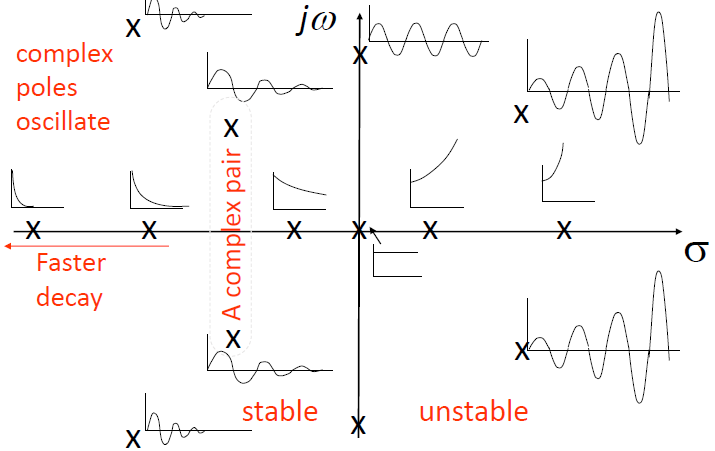
\includegraphics[width = 0.6\textwidth]{../img/diagram93.png}
\end{figure}
\end{document}